
Machine learning is the a of computer science where the computer uses a set of algorithms to learn properties from a given data set $\mathcal X$. The first machine learning problems (1950s) involved learning a function $f: \mathcal X \to \mathcal Y$ that mapped an input $x \in \mathcal X$ to a label $y \in \mathcal Y$. This discipline is commonly known as \emph{supervised learning}.

In the 1970s \emph{backpropagation} was developed, allowing networks to adapt to new situations. Since then, diverse algorithms that manage to find truly complex $f$ functions have been developed and new problems have emerged. Supervised learning has a huge cost (economic, time): all the examples in the dataset must be labeled. This is so expensive due to the  the fact that labeling examples is a slow process, and has to be done mostly manually. 

\emph{Unsupervised learning} avoids this problem by trying to infer properties of the data using the \emph{unlabeled} dataset. By not needing to have the labels of the examples, companies can save money and time that they would have invested creating a label for each individual example.

When the dimension of the data is high, for instance when treating images computationally, it is usual to first create a \emph{representation} of the input data. Combining this idea with unsupervised learning, we reach to the field of \emph{representation learning}, which studies how to create representations of the data that are useful for performing other tasks such as classification.

Ideally, we would like the original data and the representation created to contain the same information. A way of measuring this is using the \emph{mutual information} $I(X,Z)$ between the input $X$ and the representation $Z$. The mutual information is expressed as:
\[
I(X,Z) = H(X) - H(X|Z),
\]
where $H(X)$ is the entropy of $X$ and $H(X|Z)$ is the conditional entropy.

\begin{figure}[H]
    \centering
    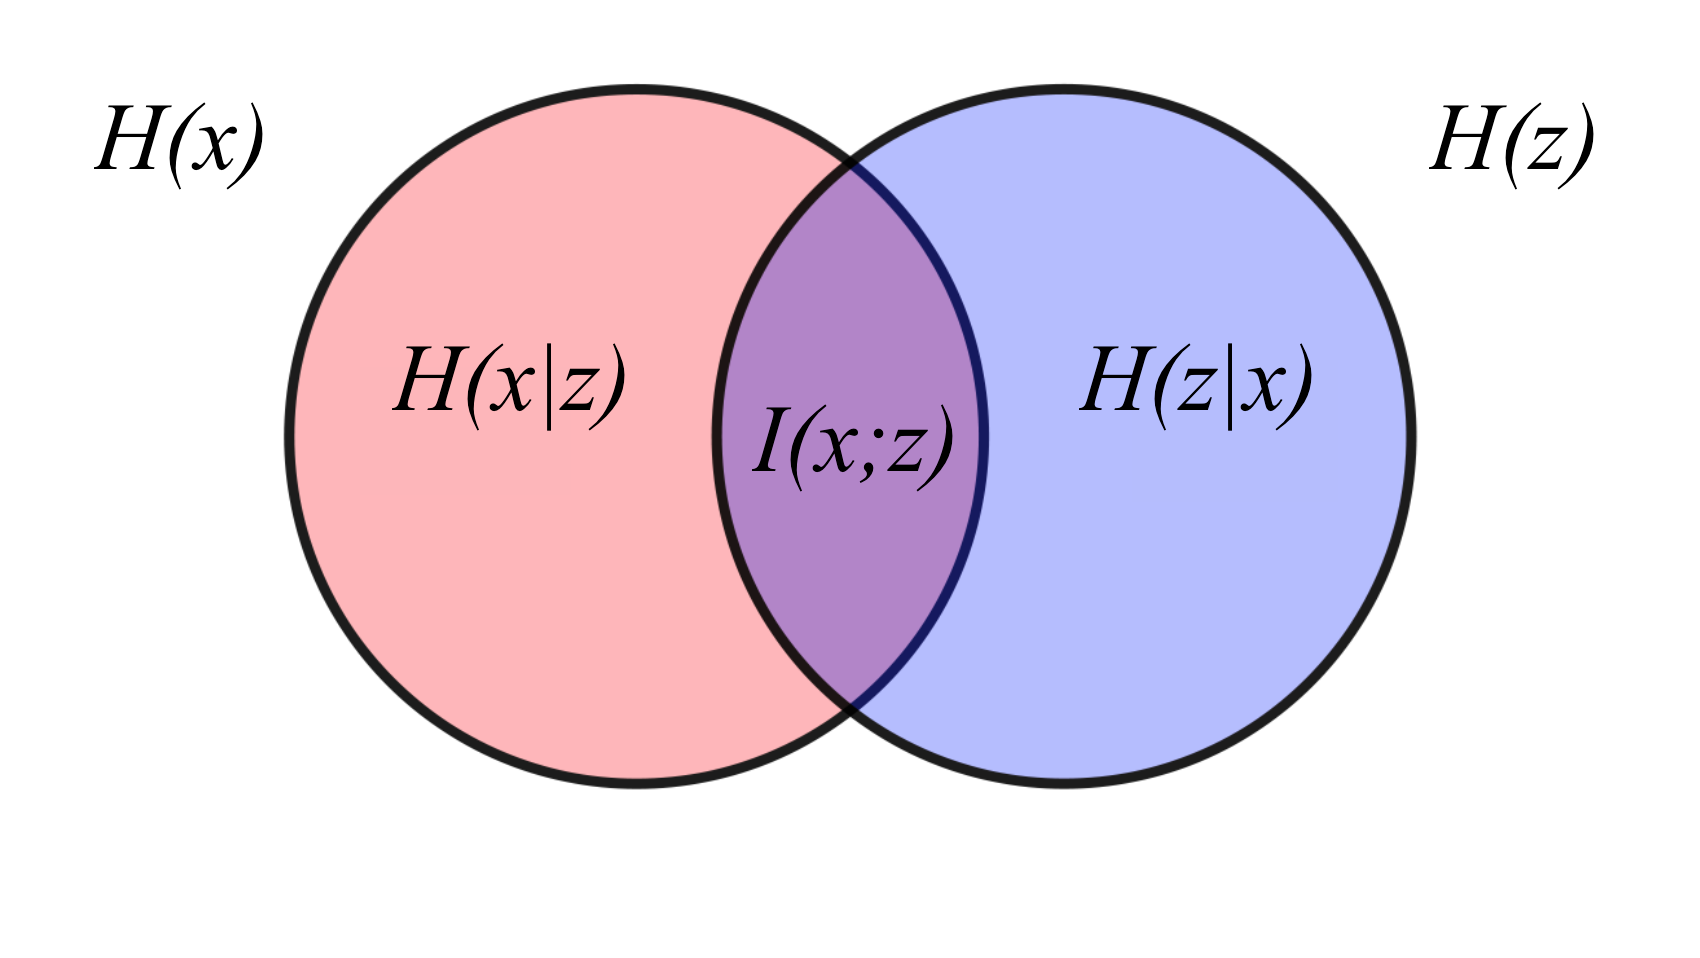
\includegraphics[scale=0.25]{mutual-info}
    \caption{Venn Diagram showing the relationships between the entropies and the conditional entropies of random variables $X$ and $Z$.}
\end{figure}

Since the entropy is a way of measuring ``\emph{how surprising is that an event occurs}'' (this is explained in this document), intuitively the mutual information measures the decrease of uncertainty that we obtain in $X$ when we know that $Z$ has occurred.

Calculating the mutual information between two variables, however, is not an computationally easy problem. Because of this, a way to approach the mutual information maximization is by obtaining lower bounds and maximizing them. Although a few more bounds are proved in this document, we remark the \emph{Contrastive Lower Bound} on the mutual information, which is expressed as follows:
\[
I(X,Z)  \geq - \ell(\theta) + \log N,
\]
where $\ell(\theta)$ refers to the contrastive loss. In short, the \emph{contrastive learning} problem consists of, given elements obtained from one distribution $P$ (considered as positive samples) and elements obtained from a different distribution $Q$ (considered as negative samples), learning how to discriminate between the elements of the different distributions. In order to do this, the recently mentioned contrastive loss is used, which usually takes the form
\[
\ell_{i,j} = -  \log \frac{f(x_i,x_j)}{\sum_{x_k \in X}f(x_i,x_k)}.
\] 
Intuitively, contrastive loss takes the output of the network for a positive example and calculates its distance (using the function $f$) to an example of the same class and contrasts that with the distance to negative examples. In other words, the loss is low if positible examples are encoded to similar representations and negative examples are encoded to different representations. The use of this contrastive loss maximizing the mutual information had a huge impact on the state of art results of representation learning in 2018 \citep{oord_representation_2019}, achieving very promising results.

However, during the development of this work (around July 2020), this drastically changed. New papers  \citep{chen_simple_2020, grill2020bootstrap} appeared stating that the success of the methods that were maximizing mutual information between the input and its representation was not caused by mutual information, but by the specific form that the contrastive loss has.

With this papers, new frameworks for representation learning appeared. These frameworks provided an ingenious way to apply  the contrastive learning set up to representation learning. This technique consists of presenting different perspectives of the same image to two different encoders (the neural networks that learns how to transform the input to a representation) different \emph{perspectives} (or, being technical, \emph{data augmentations}) of the same image and, later, trying to minimize some sort of distance between these views.  

To achieve this, these perspectives are obtained by applying transformations to the original image. It is shown that the chosen transformations and how to sequence them before passing the transformed image to the neural network really affects the performance of the models.

All this considered, the interest of this work  speaks on its own. Being able to train networks that learn representations that are good enough on its own to perform downstream tasks without needing the supervision of having the labels of the data opens a world of possibilities in many areas. For instance, many insurance companies need to pay their workers to label large amounts of  different insurance bills that they offer to their clients. With the advances presented in this work, these companies would only have to label a very small amount of images to be able to classify the representations obtained by the frameworks.


\section*{Main goals and results achieved}

The main goals of this bachelor's thesis were:
\begin{enumerate}
\item To study, understand and present the basic concepts and properties of \emph{mutual information}, which is in the field of \emph{Information Theory.} Also, related to this, to present some lower bounds that can be used to maximize the mutual information between two random variables.
\item To study the \emph{noise contrastive estimation} problem, and how it is applied to machine learning.

\item To test the most important frameworks that achieve the current state of art results in representation learning. 
\end{enumerate}

The first two goals were successful. For the latter goal, two different frameworks were tested: \lstinline{SimCLR} and \lstinline{BYOL}. 

Different executions were made for each one, trying to find the set of parameters for being able to obtain a high classification accuracy on a specific dataset. The selection of the chosen hyperparameters was argued and the limitations and problems we face are also presented. This way, I gained not only a deep understanding of the representation learning problem and how it is solved, but also in computational capability of the used hardware, so that a plausible future plan could be to improve the results obtained by making use of even better computational resources.
